\chapter{System Design}\label{ch:design}

\section{Architecture}
% ADR 0002: what runs in fall, what is deferred to spring and why.
\todo{Component diagram: web client, FastAPI, PostgreSQL with pgvector, source snapshots;
spring: job queue, AI service.}

\section{Requirement data and rule schema}
Requirements are data, not code. A destination's rule set is the EU baseline plus one national
layer; every checklist item and rule cites a source passage, and the loader rejects files whose
sources, documents, fields or field types do not match.
\todo{Rule kinds table (data/requirements/README.md) and one YAML example in a listing.}

\section{Data model}
\todo{ER diagram exported from docs/design/data-model.md; principle: YAML is the source of truth,
the database keeps versioned copies so every finding can be explained later.}

\section{Source monitoring}
\todo{Snapshot pipeline, manifest, administrator approval, notification of affected files only.}

\section{User interface}
The interface is one responsive web application with Turkish and English text
(Figure~\ref{fig:ui-checklist}; all screens in Appendix~\ref{app:screens}).
\begin{figure}[ht]
  \centering
  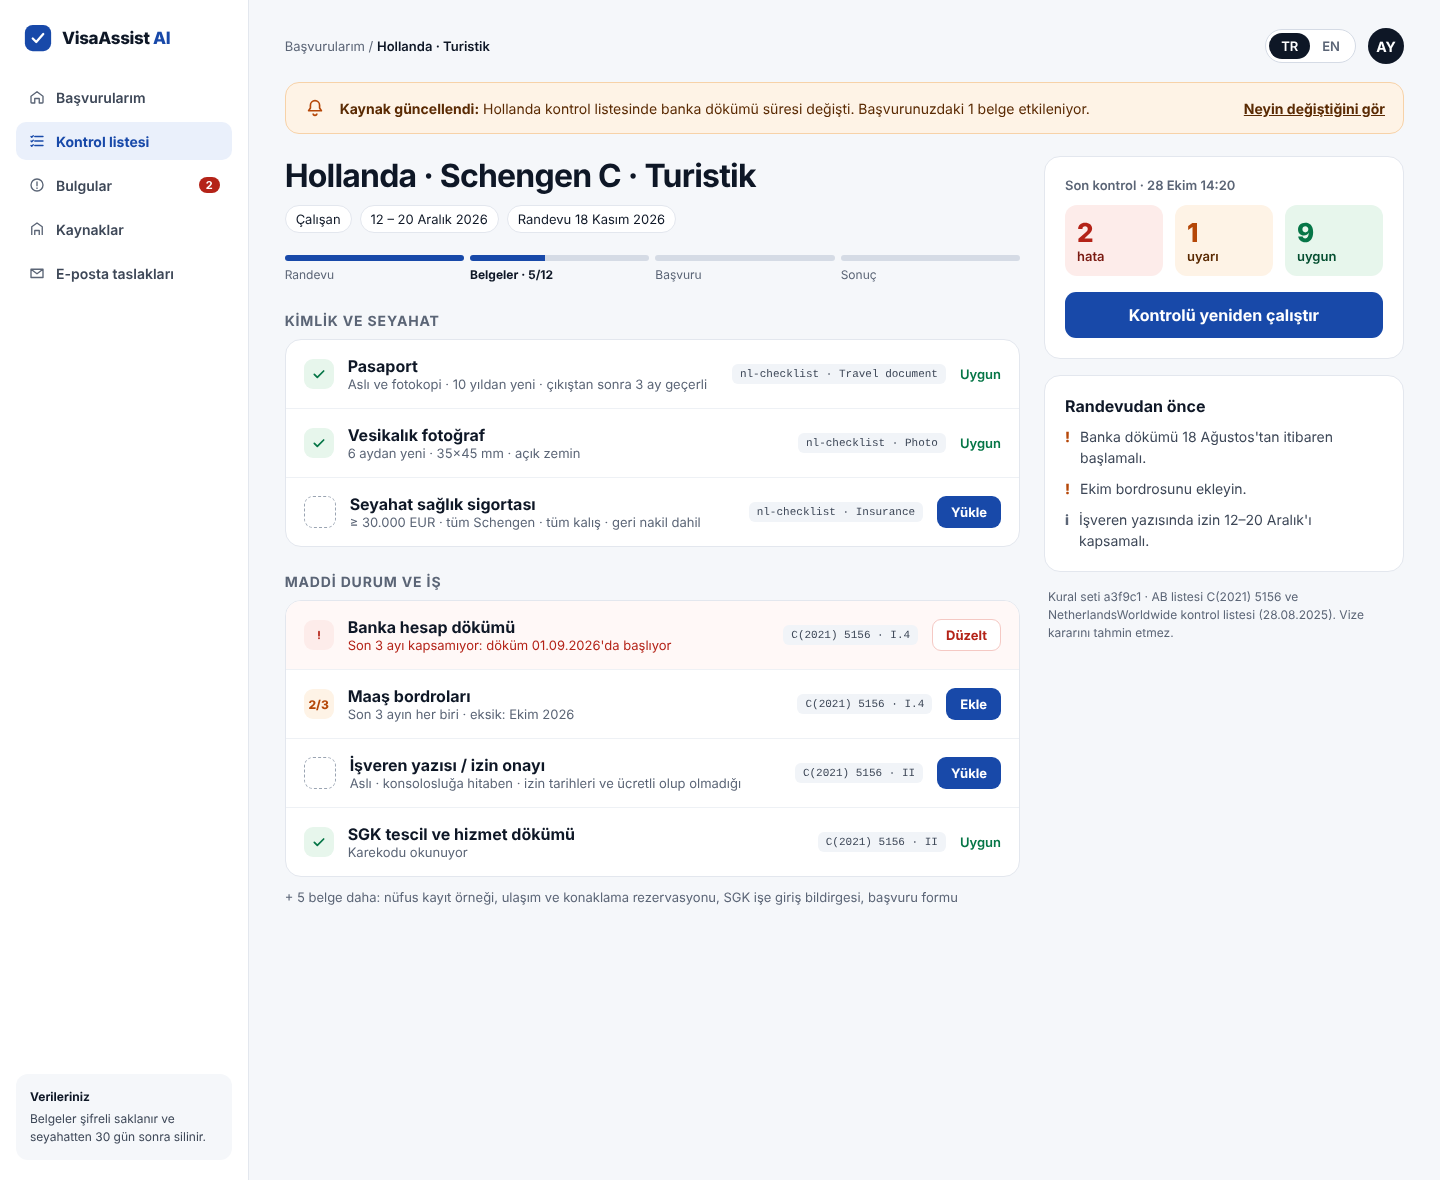
\includegraphics[width=\textwidth]{02-web-checklist.png}
  \caption{Application checklist: status, source tag and one action per document.}
  \label{fig:ui-checklist}
\end{figure}

\section{AI components and cost (spring)}
\todo{ADR 0003: model per task, four-layer cost control, estimates checked against measurement.}
